\ifpdf
    \graphicspath{{Chapter9/Figs/Raster/}{Chapter9/Figs/PDF/}{Chapter9/Figs/}}
\else
    \graphicspath{{Chapter9/Figs/Vector/}{Chapter9/Figs/}}
\fi

\chapter{The Politics of Toxicity in Content Moderation Infrastructures - under review @ New Media and Society}\label{chap:filter}
\zw{In collaboration with Nanna Bonde Thylstrup (who's the first author)}

Throughout our process, we have worked with notions of ``toxicity'' and ``abuse'' without further examining their implications or the political constructs they live within. Here we then take a critical look at the implications of the political economies which these terms live within and how content moderation infrastructures define toxic content.

Through an examination of three content moderation tools, the Perspective API, Opt Out and our own abuse detection system from \autoref{chap:liwc}, we argue that content moderation's historical reliance on static categories, which are embedded in social systems of racism and patriarchy, embeds content moderation technologies in structures that risk reproducing social inequalities. We choose the three technologies to illustrate the differences between top-down and bottom-up approaches to content moderation and the distinct ways in which they engage in embed meaning to ``toxic'' and ``abuse'', and the cultural filtering work that content moderation has come to do. These three examples enable to us identify the challenges inherent in attempts to automate and scale content moderation and ask two fundamental questions of content moderation: Whom are content moderation systems for and who gets to define and enforce them?

By engaging with scholarly work that draw on and develop pollution and discard theory, we can better understand this discourse of ``toxicity'' and identify new avenues of research for content moderation studies. Moreover, by relying on theories of social pollution from anthropology \cite{Douglas:1966} and work on dirt and toxicity in the field of discard studies \cite{Libeoiron:2018,Lepawsky:2019}, we argue that content moderation should move beyond the question of merely removal of toxic content to a productive 're-ordering of our environment' through practices of classification and purification \cite{Douglas:1966}.

\section{Content Moderation as a Problem of Dirt}
If we consider content moderation technologies as `protective' filtering systems that reject and accept to ensure the `health' of communities, then we must also reckon with their inseparability from discourses of hygiene and pollution. By conceptualising content moderation systems deployed with the purpose of protecting platforms and their communities against existential threat that occurs through the through the existence of dirt \cite{Lepawsky:2019}, we can begin to develop an understanding of online abusive content as `toxic'. Thus, content moderation systems become complex processes which aid the communities, or platforms in their practice of self constitution.

By applying \citet{Douglas:1966} to content moderation technology and their classification schemes of harmful and abusive content, we find that content moderation requires constant efforts to classify, detect, and reorganise content online in every step of the process. From conceptual frameworks and annotation guidelines to computational models and from organisational systems to manual labour. Each of these elements of the content moderation system become different mechanism that allow the system to exert efforts to positively reorganise online environments through sanctioning content. In many online spaces, e.g. Facebook's familiar space of people you (have once) know(n) content moderators are hard at work, removing human rights abuses and system critiques alike. In such cases, removal is not only a negative act, but also a part of productive processes embedded in complex community formation that reconstitute the platforms they operate on.

Douglas' framework of dirt allows us to see and examine the cultural embeddings of content moderation. Considering such cultural embeddings, it is no surprise that operationalising terms such as `toxic', `hate speech', and `offensive' lead to negotiations between coders and designers of data \cite{Waseem:2016}. Such issues with operationalisation of the terms then also blur the decision boundaries learned by machine learning for content moderation. Moreover, in spite of such culture wars in the data annotation processes and their downstream effects on blurring machine-identified decision boundaries, many machine learning methods are presented with the result of the annotation process as objective truths. The machine learning methods applied to such would-be objective bodies of data codify the patterns and correlations with the associated labels. What was once subjective is then presented as objective, universally true rules, as machine learning methods play the God Trick.\vspace{5mm}

Faithful representations of collective negotiations of what constitutes `toxic' or `abusive' must then also have a degree of indeterminability to them. This indeterminability of labels is then an indication of the instability of the terms and their operationalisations. It follows then, that indeterminability can cause harm to social order \cite{Hall:1997} as multiple concurrent decoding processes may exist that deviate from the intended encoding. In the setting of content moderation, we must add an intermediary in Hall's \cite{Hall:1997} setting of encoding-decoding framework, as the content moderation system itself must decode and adjudicate a decision: Should this content be actioned or not? Through answering this question, the meaning made in the decoding process of the content moderation system then becomes the final decision on its meaning, regardless of its intended encoding or the decoding of the reader.

Understanding these meaning-making processes and positions of power allows us to recognise that some content might be flagged as problematic because of its `inability to be assimilated into existing socio-cultural categories and systems' \cite{Rafi:2015}. In handling content for which multiple concurrent and contradictory meanings are made, content moderation should be a relative practice that constantly oscillates among the meanings encoded and decoded according to the context in which the actions happens. Moreover, as cultural systems can change quickly, so can the meanings of symbols. What was once accepted practice e.g. racist jokes can suddenly be considered harmful and socially transgressive; similarly what was once taboo can become acceptable practice.
Many of the issues with content moderation systems can then be traced back to these dynamic meaning-making processes, how does one determine if the usage of the N-word is used as a slur or a `soul' word \cite{Rahman:2012}?\vspace{5mm}

These dynamic complexities stand in contradiction to automated content moderation systems that assign each token a weight internally and a probability externally. These weights and probabilities are unlikely to be zero, reinforcing the assertion made by \citet{Douglas:1966}, that there is no such thing as absolute dirt. In fact, many of the methods that seek to mitigate social biases in machine learning, and by extension automated content moderation seek to re-assign weights to minimise the social marginalisation that such systems cause on already-marginalised people \cite{Liu:2019}. These mitigation strategies frequently operate within positivist logics of optimisation. The aim of such re-ordering within automated content moderation systems is not to remove all traces of social biases within such systems, instead such works engage in a calculus of operating with minimal acceptable harms to marginalised people (see \autoref{chap:disembodied} for in-depth discussion of the impacts of such logics). However, such reordering does not take into account the unequal impacts of equal treatment (see \autoref{chap:socialscience} for a deeper discussion on the impacts of equality based systems in an unjust world). In fact, such work rarely takes into account that through their search for patterns to aid in prediction, automated systems may go beyond simply representing inequities and instead actively amplify them.\vspace{5mm}

The fact that human, machine, and hybrid content moderation systems reproduce such social inequities has been the object of both scholarly work \cite{Davidson:2019,Sap:2019,Dixon:2018,Gomes:2018} and public criticism \cite{Guynn:2019}. Indeed the excessive policing of marginalised communities has given rise to the use of POTs \cite{Kulynych:2020} in efforts to circumvent such policing through a number of tactics including phonetic spelling (e.g. the use of `wypipo' instead of `white people') \cite{Guynn:2019}. These methods of circumventing content moderation systems come from the experience of negative removals \cite{Guynn:2019}. Examples of such negative removals. Considering, for instance, content moderation of AAE, the content moderation filters may reproduce racialised logics and thus excessively reject content written in AAE as particularly dirt-like. At other times, the system may fail to capture the semantic richness of AAE. For many content moderation systems, the working assumption embedded in the systems  \cite{Davidson:2019} that is curated through labelled data \cite{Sap:2019} is that any mention of the n-word invokes a negative stereotyping \cite{Waseem:2018}. However, as \citet{Rahman:2012} reminds us, beyond the negative uses of the n-word as a slur, there is a rich and complex cultural history and meaning assigned to the word, when it used by in-group speakers. Such structural biases occur because in efforts to scale the size of data, working with `deep data' (Lori Kendall cited in \citet{Brock:2015}), i.e. working on data with methods that include deeper insights about the `cultural, moral, and social choices about technology use' found in different cultural communities \cite(Brock:2015}.

Thus, in particular for the moderation of language, many content moderation infrastructures reproduce the problems of respectability politics and its favouring of upper-middle class White ideals \cite{Kerrison:2017}.

\section{Addressing Toxicity Online}

Through the exemplification of Jigsaw's Perspective API and Opt Out's browser-plugin, we examine the issues of power differentials, respectability politics, and the complex space in which content moderation systems navigate.

\subsection{Perspective}

The Perspective API was developed \cite{Wulczyn:2017} and launched by Jigsaw and Google's Counter-Abuse Technology team in 2017. The method employed by Perspective aims to explore online discussions through experiments, models and research data in order to create better governance tools and `explore strengths and weaknesses of [machine learning] as a tool for online discussion'. The API is developed then to score the toxicity of provided text using machine learning. Each bit of text, or comment is then given a score between zero and one, where a toxicity score that is greater than or equal to $0.9$ are considered toxic.

In order to identify what is toxic and not toxic, Perspective offer defining a toxic comment as ‘a rude, disrespectful, or unreasonable comment that is likely to make you leave a discussion' \cite{PerspectiveAPI}. This definition is used in the data creation process. The data is created `asking people to rate internet comments on a scale from “Very toxic” to “Very healthy” contribution' \cite{Gomes:2018}. As the definition is decidedly ambiguous, a certain degree of the different internal operationalisations of the definition, and thus the underlying dataset, is then informed by the people who trained the machine learning underpinning the API. The API works in real-time allowing for people to see the toxicity score of their comment as they are typing. The function of Perspective, phrased in terms of dirt is then to distinguish between the `toxic', which threaten the stability of online discussions, and the `healthy', that the communities can reinforce themselves around.\vspace{5mm}

In its description, as well as in the labelling choices, Perspective conceptualises toxic in opposition to healthy, or in terms of \citet{Douglas:1966}: dirty and clean. However, unlike many other datasets, the training data underpinning Perspective is not only trained on found objects that are then annotated, the dataset also consists of crowdsourced abusive comments that were generated by antagonist users trying the system \cite{Marvin:2019}. \vspace{5mm}

The Perspective team note that `initial testing revealed major blind spots and algorithmic bias` \cite{Marvin:2019} which were then addressed, however as librarian Jessamyn West discovered such biases had not been fully addressed (see \autoref{fig:jessamyn}); examples such as `I am a man' produced a toxicity score of only $0.20$ while `I am a gay black woman' scored $0.87$, that is just below the threshold of being deemed as toxic by the system.

\begin{figure}[h]
  \centering
  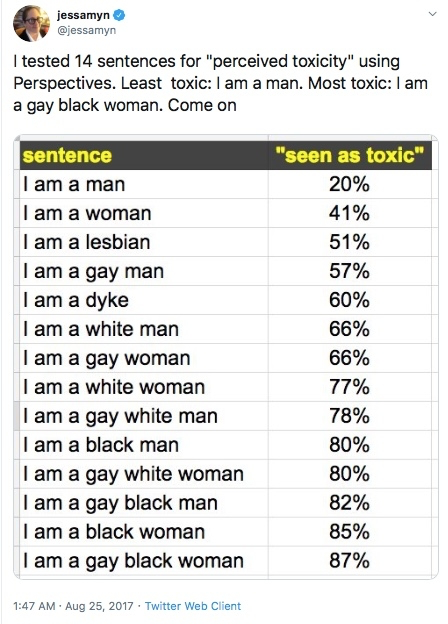
\includegraphics[scale=0.5]{Jessamyn.png}
  \caption{Jessamyn West on Twitter.}
  \label{fig:jessamyn}
\end{figure}

Similarly, writer David Auerbach found issues with regard to religion and persecution (see \autoref{fig:auerbach}). For instance, he found that the model predicted a toxicity score of $0.73$ for the statement `whites and blacks are not inferior to one another', $0.70$ for `hitler was an anti-semite', and only $0.18$ for ``some races are inferior to others', $0.06$ for `Hitler's biggest mistake was not getting the job done' , and $0.05$ for `14/88' a common neo-Nazi symbol.\footnote{Please see https://www.adl.org/education/references/hate-symbols/14-words and https://www.adl.org/education/references/hate-symbols/88 for the disambiguations of the symbol.}

\begin{figure}[h]
  \centering
  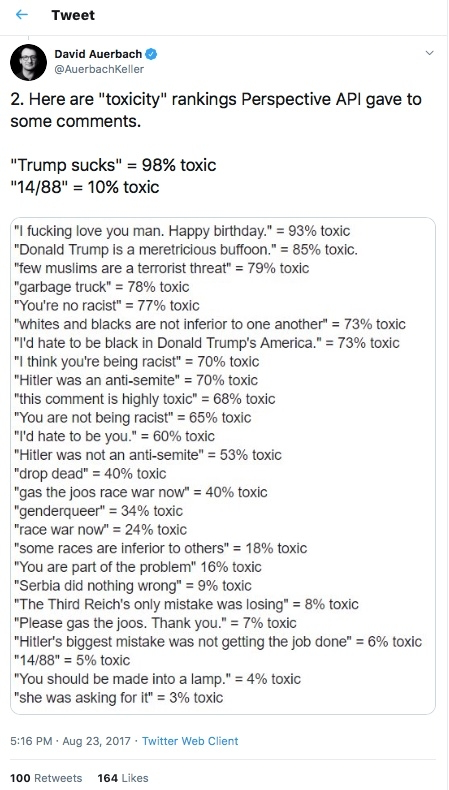
\includegraphics[scale=0.5]{auerbach.png}
  \caption{David Auerbach on Twitter.}
  \label{fig:auerbach}
\end{figure}

Such discrepancies in toxicity scores reproduce oppressive gendered, racial, and sexual hegemonies which assign negative attributes to deviations from straight, male, and white identities while assigning neutral or, in the worst and most likely case, positive values to information maintaining such hegemonies even at the cost of promoting fascist views. Why did Perspective then learn such oppressive logics of racism, anti-Semitism,, sexuality, and gender? The answer is likely to be found in the data the model is trained on as well as how the machine learning model is likely to function.\vspace{5mm}

We delineate between three different causes: 1) the training data, 2) the word-embeddings used for the model, and 3) the model behaviour itself. First, the training data is likely to consists of imbalanced distributions of identity words in the different classes. It is highly likely that terms such as `black', `gay', and `woman' more frequently occur in the positive classes than in the negative class, for this reason the model is likely to learn stronger correlations between those identity terms and the positive classes than `white' and `man'. The occurrence of the terms documented by Jessamyn west in a document parsed by the API is then more likely to produce the label `toxic'. Conversely, content that uses `civilised' language while arguing for positions that more profoundly disturb the social order are a) less likely to be labelled as toxic by virtue of their `civilised' language and b) less frequent in the data overall, leaving seemingly benign words used in a context the model has rarely seen, and will therefore not know that it is in fact `toxic' language that needs `cleaning up' \cite{Gomes:2018}.

Second, through the application of GloVe word embeddings \cite{Pennington:2014} as these allow for the machine learning model to take advantage of knowledge held outside of the training data. Several works have identified that severe social biases against marginalised communities are apparent in word embeddings \cite{Speer:2017,Bolukbasi:2016,Nissim:2019,Zhao:2017,Zhao:2020}, moreover even once such embedding spaces have been treated for social biases they continue to exhibit social biases \cite{Gonen:2019}. Thus, the external knowledge that the model relies in is then also likely to exhibit characteristics of oppressive racial, sexual, and gendered social structures.

Finally, the model architecture itself is a likely culprit of amplifying the biases held within the dataset and word embeddings \cite{Zhao:2017}. As machine learning models seek to identify decision boundaries between the different classes, between the dirt and the clean, the models seek to determine boundaries in the contextual and indeterminable. Therefore, the models learn strong correlations with what is most frequently in the positive classes, what is most frequently in the negative classes, and what is frequently in both positive and negative classes. It is in the final space that the decision boundaries are drawn, however social biases are likely to be seen in spaces further away from the decision boundaries, more towards the positive and negative classes respectively. It is in the `civilized' language production tending towards the negative classes that some socially disturbing content is found, and it is towards the space of the positive classes that find strong correlations with mentions of marginalised identities.\vspace{5mm}

As Jigsaw have stated their commitment to treat their models for social biases \cite{Marvin:2019}, we can assume that some development may have happened since Auerbach and West's examinations. However, at the time of writing w find that the phrase ‘black queer women’ scored 0.77 toxicity, while ‘white men are’ scores 0.25, and ‘white straight men are’ scored 0.50.

\subsection{Opt Out}
Our second case study is Opt Out, an open-source Firefox browser extension founded by Theresa Ingram. The extension, which was launched on the 8th of March, 2020, focuses on detecting misogyny. Opt Out define misogyny as `any verbal, visual or physical harassment and abuse rooted in misogyny that is threatened, carried out and/or amplified online' \cite{Ingram:2020}. Unlike the Perspective's aim to address content moderation at the platform level, the aim of Opt Out is to empower individual users to address the torrent of misogyny from their own timeline. Thus, while Perspective aims to provide a globally prescriptive understanding of `toxic', Opt Out aims to adjust to each individual's tolerance of misogyny, under a global understanding of what constitutes misogyny. The downstream impacts of this distinction includes how power is distributed. In Perspective's centralised architecture, it retains the power to identify and distinguish what is dirt and what is not. In Opt Out's model, the definitional power is held by Opt Out, as with Perspective, however distributes that power to their users, as they allow for users to set how the dirt found is handled.

\begin{figure}[h]
  \centering
  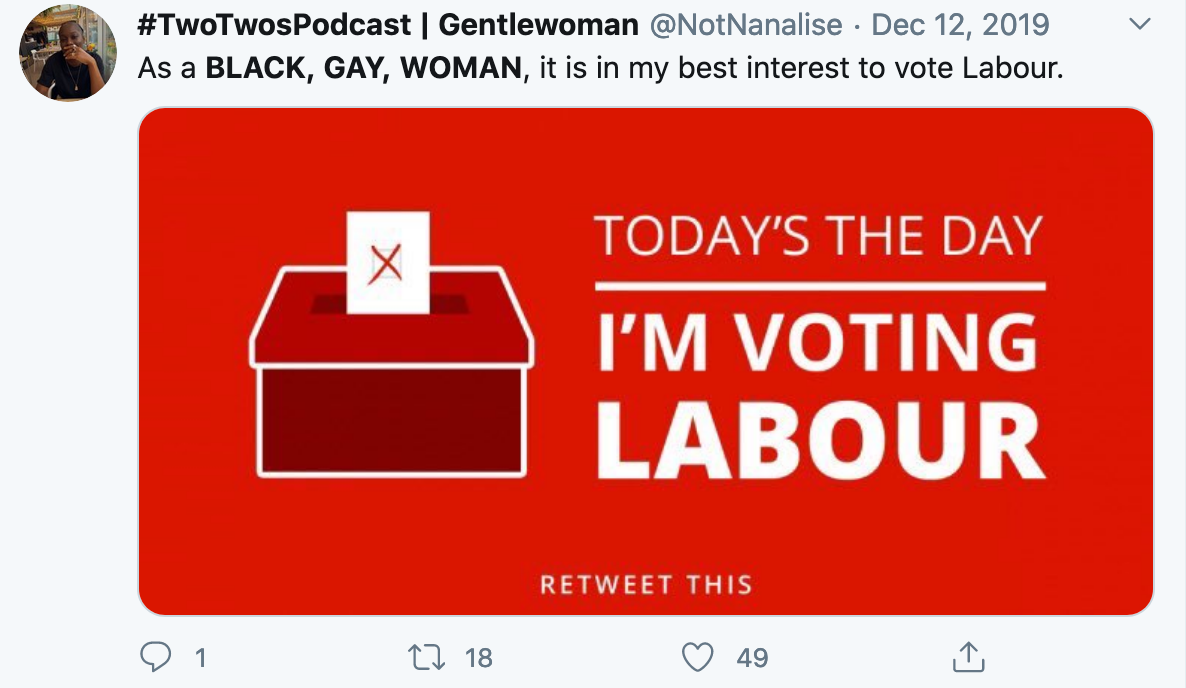
\includegraphics[scale=0.5]{Notnalise.png}
  \caption{NotNalise on Twitter.}
  \label{fig:notnalise}
\end{figure}

Foregrounding the cultural contingency of harmful expressions, Opt Out implement machine learning systems that are trained on multiple previously published datasets with competing definitions and operationalisations of misogyny, thus countering essentialist tendencies at the cost of model performance.

\begin{figure}[h]
  \centering
  
\includegraphics[scale=0.5]{Rona.png}
  \caption{Flash\_Hoe on Twitter.}
  \label{fig:flash_hoe}
\end{figure}

Considering \autoref{fig:flash_hoe} and \autoref{fig:aquaria}, we see tensions in how to understand, or decode the term `b**ch' to distinguish between pejorative and reclaimed uses of the word. Further, while there is a distinction in the text-only reading of the two tweets, by considering the image accompanying them, it is clear that the pejorative use in \autoref{fig:flash_hoe} is in fact referring to a non-human entity, namely the respiratory virus COVID-19. This depiction of the virus then hedges the pejorative nature of the text. In contrast, the image used in \autoref{fig:aquaria} figures as underscoring the point, and the positive nature, of the tweet. These uses of images as an additional modality of communication in the tweets exemplify the incomplete natures of identifying dirt in a single modality. Where the image in \autoref{fig:flash_hoe} negates the pejorative message in tweet, \autoref{fig:aquaria} brings more emphasis to the message.

\begin{figure}[h]
  \centering
  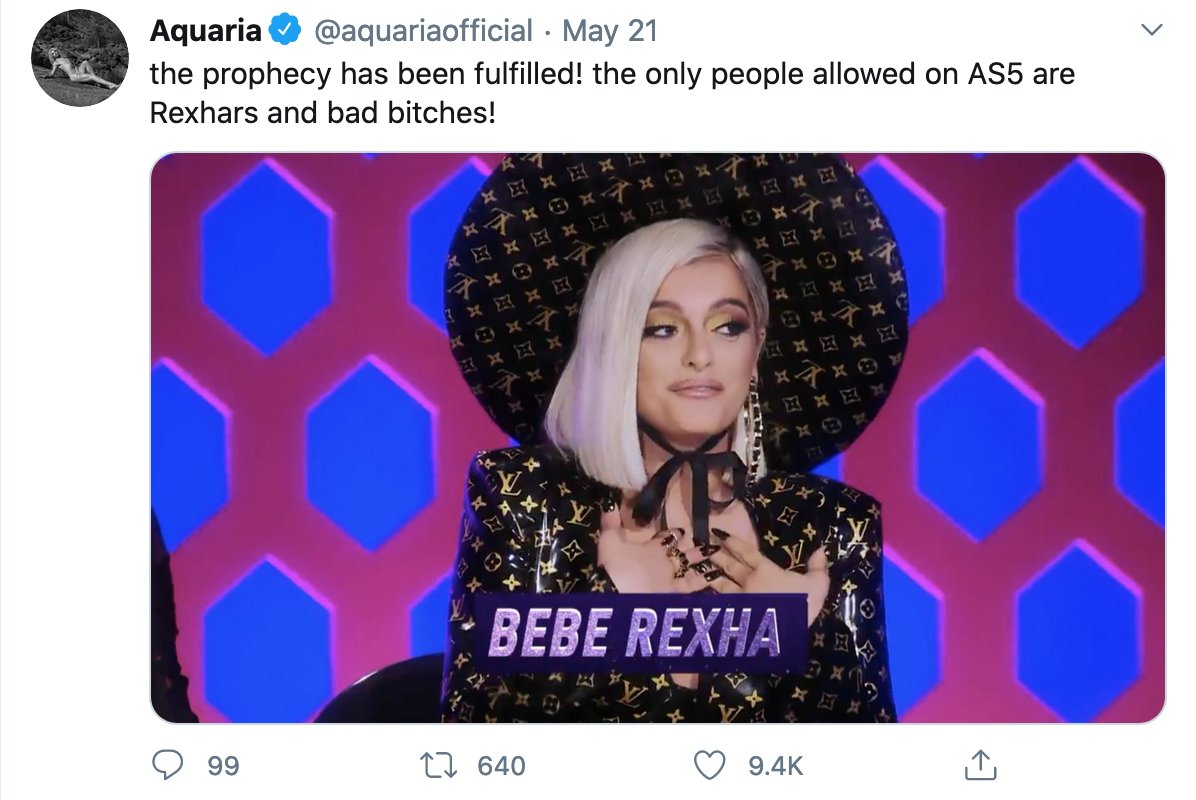
\includegraphics[scale=0.5]{aquaria.png}
  \caption{Aquaria on Twitter.}
  \label{fig:flash_hoe}
\end{figure}

Moreover, considering \autoref{fig:notnalise} we see that identity terms, even compounded ones, are not punished by Opt Out. This suggests that the different understandings within the distinct datasets used to train the model may not have strong correlations with identity terms and the positive class. However, as the developers of the extension have shared, balancing the different understandings and levels of allowable misogyny does not come without its own costs. As machine learning systems rely on consistency in data and annotation to identify decision boundaries between different bodies of labelled data, there are seemingly spurious inconsistencies in what the model deems harmful, which has a downstream effect on the users who may experience what appear to be random effectiveness of the model in removing misogyny from their streams. Opt Out's use of multiple datasets and competing definitions of misogyny then penalises the dataset underpinning the model's positive class as the different datasets have different annotation schemes and define misogyny in closely related, yet distinct ways. Considered through \citet{Douglas:1966} framework, we can understand this inconsistency, or noise less as a technical problem to be optimised for or solved, but instead as a fundamental cultural quesiton of boundary setting and tolerance for ambiguity. Such ambiguity in the training data create competing signals for the model, as it seeks out correlations to rely on to identify misogyny. Further, as the model is trained on multiple competing definitions, it is limited in the nuances of any single operationalisation of misogyny; consequently a sparse modelling space is made more sparse, as less data remains at the centre and more is pushed to the margins of the space. The data, and correlations that remain at the centre then tend to consist of highly normative understandings of what is and what is not dirt.

\section{The Deeper Politics of Toxic Discourse in Content Moderation}

Considering then the perspectives on toxic offered in \cite{Risam:2015}, we can try to understand these cultural-technical issues that are encountered by Perspective and Opt Out in their aims to distinguish between dirt and not dirt.

\section{Concluding Remarks}
